\documentclass[12pt, letterpaper]{article}
\usepackage[utf8]{inputenc}
\usepackage{titlesec}
\usepackage{graphicx}
\usepackage{mathtools}		% For piecewise functions



\titleformat*{\section}{\normalsize\bfseries}
\titleformat*{\subsection}{\small\bfseries}
\titleformat*{\subsubsection}{\small\bfseries}
\titleformat*{\paragraph}{\large\bfseries}
\titleformat*{\subparagraph}{\large\bfseries}

\begin{document}
\begin{center}
\Large DSA/ISE 5113 Advanced Analytics and Metaheuristics
\Large Homework \#4\\
\vspace{3mm}
\normalsize April 5, 2020\\
\vspace{3mm}
\normalsize Rachel Bennett
\end{center}

\section*{Question 1}
\subsection*{(a)}
The facility location problem consisted of a set of $I$ districts that needed to be served by firehouses in possible sites $J$. 
Our formulation uses:

\[
  y_j =
  \begin{cases}
                                   1 & \text{if site $j$ is selected} \\
                                   0 & \text{otherwise} \\
  \end{cases}
\]


\[
  x_{ij} =
  \begin{cases}
                                   1 & \text{if district $i$ is assigned to site $j$} \\
                                   0 & \text{otherwise} \\
  \end{cases}
\]

Each district should be assigned to exactly one firehouse.

$$ \sum_{j=1}^{J} x_{ij} = 1 \text{   ($i$ = 1, 2, ..., $I$)}$$

No district should be assigned to an "unused" site.

$$ \sum_{i=1}^{I} x_{ij} \leq y_{j}I \text{   ($j$ = 1, 2, ..., $J$)}$$

It is important that either at least sites 1 and 2 or sites 3 and 4 are selected. This is done through another binary variable $z$.

$$y_1 + y_2 \geq 2z$$

$$\text{or}$$

$$y_3 + y_4 \geq 2(1-z)$$

A new variable was created for each site to denote the population that would be serviced.

$$s_j = \sum_{i=1}^{I} p_{i}x_{ij}$$

Where $p_i$ was the population in each district. 

The total costs of servicing each site plus the cost of building each firehouse needed to stay under a given budget. 

$$ \sum_{j=1}^{J} (c_{j}s_{j} + f_{j}y_{j}) \leq B$$

Where $c_j$ is the cost of service in each district and $f_j$ is the fixed cost of building a firehouse.

The objective was to minimize the "worst-case" distances between each district center and its assigned firehouse. This was done through the creation of a variable $D$, which was set to be greater than all distances for each district $i$. 

$$ D \geq \sum_{j=1}^{J} d_{ij}x_{ij} \text{  ($i$ = 1,2,...,$I$)}$$


See attached AMPL file for code. 


\subsection*{(b)}
\subsubsection*{(i)}
The optimal solution had a worst-case distance of 31.3, using \$14,988,200 to build the firehouses and service the districts. The total 
solution time was 3.31732 seconds, with 4821 nodes explored. The root relaxation value was 6.1359. The first incumbent solution of 135.8 was found at node 121. 
\subsubsection*{(ii)}

\begin{center}
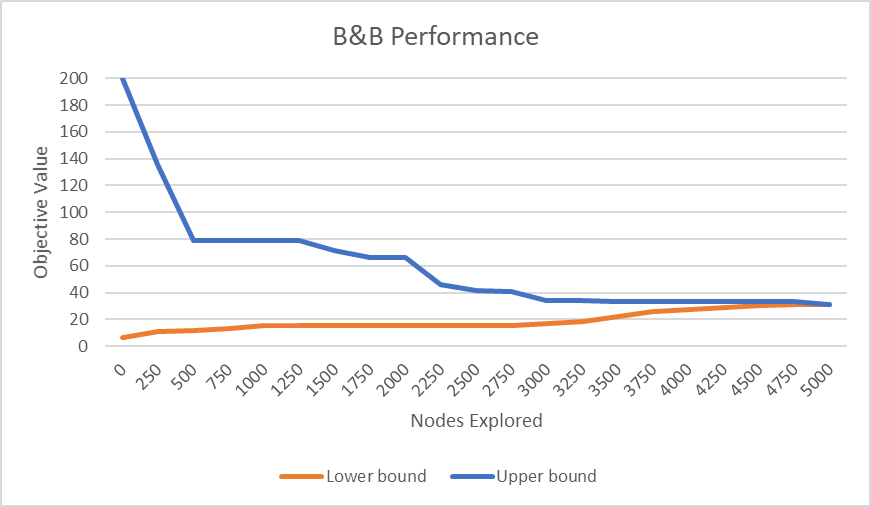
\includegraphics[scale=1]{B&B_performance}
\end{center}

As several thousand nodes were explored, the graph's x-axis was indexed at intervals of 250 nodes to reduce the size of the graph.

\subsubsection*{(iii)}

The solution time was increased slightly to 3.42617 seconds, and the enumeration tree was greatly reduced to 2706 nodes. however, the objective value stayed at 31.3, while the budget decreased to \$14,968,700.

\section*{Question 2}

\subsection*{(a)}
A potential, though inefficient, initial solution for the knapsack problem would be to either put nothing or everything in the bag. In the case of the former, it would guarentee that the closest neighborhoods would all be feasible, but it would take many iterations to get to a solution that would be even close to optimal. For the later the reverse is true - you would be likely given a solution that has a high objective value, but it would take many iterations to get to a solution that is feasible. A more efficient solution would likely be to give a probability of selection for each item in the bag, with higher probabilities giving you a fuller bag and lower probabilities for a more empty bag. This will likely take fewer iterations to find a good solution, but at the expense of potentially not finding as high an objective value as in the case of the completely full bag solution. For this program, the bag was filled randomly for the initial solution, which gave a better middle ground between high value and low number of iterations.

\subsection*{(b)}
The most intuitive neighborhood structures are variations on the flip neighborhood. For this problem, you could include a 1-flip, 2-flip, and 3-flip neighborhood structure. The 1-flip neighborhood structure would give a neighborhood of size $n$, where $n$ is equal to the number of items in the bag, while the 2 and 3 flip neighborhood structure would give neighborhoods of size ${n \choose 2}$ and ${n \choose 3}$ respectively.

\subsection*{(c)}
For solutions that are infeasible (in this case, over the weight limit), one could assign a penalty to the value of the solution. This could be done by taking the difference between the max weight and the solution's weight, multiplying by some penalty value, then subtracting this from the solution's total value. This would disincentivize the program from choosing any solutions that are over the weight limit, as they would have a low total value. In this case, the penalty value was  chosen to be the max weight of the randomly generated list of item weights. 


\section*{Question 3}

Best Improvement was implemented using the aformentioned strategies for initial solution and infeasability. The neighborhood structure used in this and all other algorithms was the 1-flip structure. 

\section*{Question 4}

First Improvement was identical to Best, but with a break statement after the first improved solution in each neighborhood was found. This caused it to run for less iterations, but it found a significantly worse solution.
\section*{Question 5}

Local Search with Random Restart was done with best improvement. The program was run over 10 restarts, with the total number of iterations coming to 71400. This version of the program had the best objective value.

\section*{Question 6}

The random walk variation of local search used the first improvement method in order to keep the number of iterations from growing too large. When the probability of a random walk was set to 50\%, it did not take an excessive number of iterations to find a solution, but the solution found was not the best. 


\section*{Question 7}

Local Beam Search was implemented with 3 neighborhoods running at the same time using best improvement. 

\begin{center}
\begin{tabular}{ l r r r r } 

 \multicolumn{5}{c}{Results} \\
 \hline
Algorithm & Iterations & \# Items Selected & Weight & Objective \\
 \hline 
Local Search (Best Improvement) & 7050 & 28 & 1499.6 & 14170.60 \\
Local Search (First Improvement) & 3055 & 16 & 1497.1 & 6391.79\\
Local Search (Random Restarts) & 71400 & 31 & 1494.6 & 15218.80\\
Local Search (Random Walk) & 6635 & 19 & 1495.1 & 7801.60\\
Local Beam Search & 12600 & 26 & 1499.3 & 11866.50\\
 \hline
\end{tabular}
\end{center}



\end{document}